
\documentclass[preview,border=0.80001bp, convert=imagemagick]{standalone}
%\documentclass{article}
\usepackage{hyperref}
\usepackage{amsmath}
\usepackage{tikz}
\usepackage{miama}
\usepackage{xcolor}
\usepackage[T1]{fontenc}

\newlength\unitlen
\tikzset{
    unit length/.code={\setlength{\unitlen}{#1}},
    unit length = 8pt
}

\begin{document}
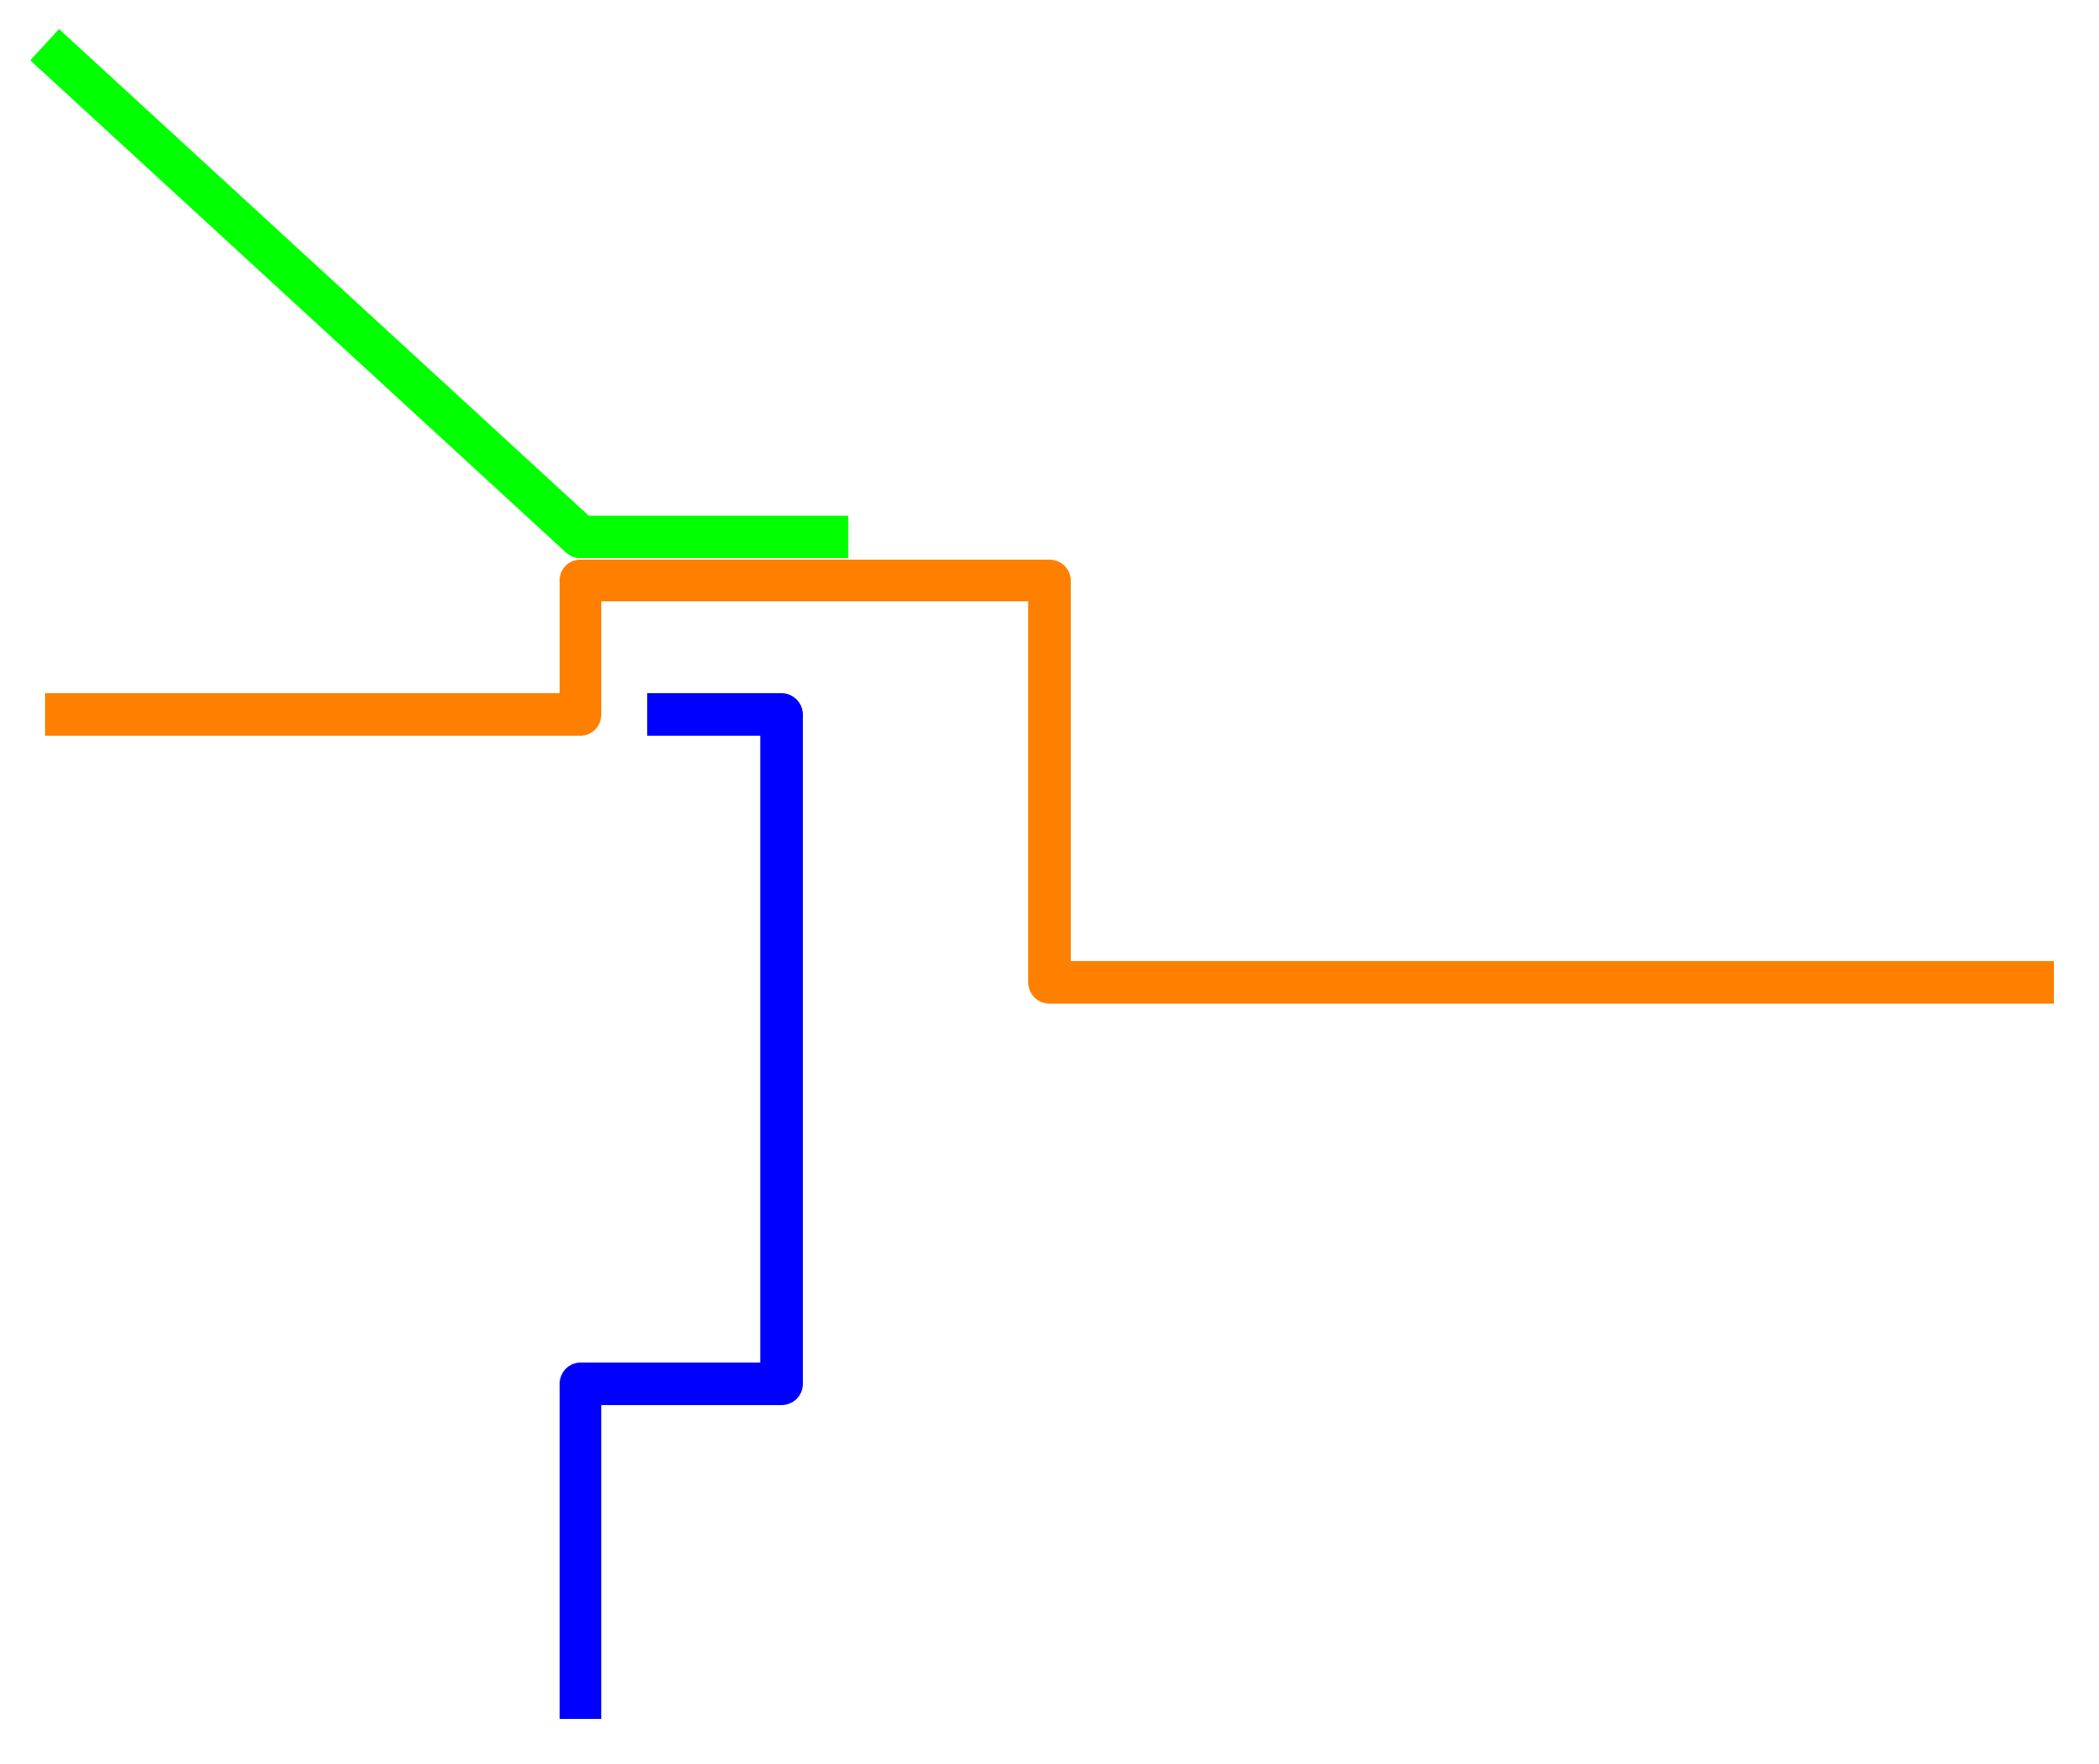
\begin{tikzpicture}[line width=18pt]
    \draw[line join = round, color=orange] 
    (-15,0) -- (-7,0) -- (-7,2) -- (-3,2) -- (0,2) -- (0,-4) -- (15,-4);

    \draw[line join = round, color=green] 
    (-15,10) -- (-7,2.65) -- (-3,2.65);

    \draw[line join = round, color=blue] 
    (-7,-15) -- 
    (-7,-10) -- 
    (-4,-10) -- 
    (-4, 0)  --
    (-6, 0)
    ;

%j    \node[minimum size =9mm, circle,fill=black] (c) at (1,0){};
%j    \node[minimum size =8mm, circle,fill=white] (c) at (1,0){};
%j    \node[minimum size =4mm, circle,fill=black] (c) at (1,0){};
%j    \node[circle,fill=white] (c) at (1,0){};
\end{tikzpicture}
\end{document}

